\documentclass{article}
\usepackage[utf8]{inputenc}

% Code packages and configurations
\usepackage{color}
\usepackage{float}
\usepackage{graphicx}
\usepackage{listings}
\usepackage{url}

\definecolor{dkgreen}{rgb}{0,0.6,0}
\definecolor{gray}{rgb}{0.5,0.5,0.5}
\definecolor{mauve}{rgb}{0.58,0,0.82}

\lstset{frame=tb,
  language=Java,
  aboveskip=3mm,
  belowskip=3mm,
  showstringspaces=false,
  columns=flexible,
  basicstyle={\small\ttfamily},
  numbers=none,
  numberstyle=\tiny\color{gray},
  keywordstyle=\color{blue},
  commentstyle=\color{dkgreen},
  stringstyle=\color{mauve},
  breaklines=true,
  breakatwhitespace=true,
  tabsize=3
}

\title{People Recognition}
\author{David Suárez}
\date{\today}

\begin{document}

\maketitle

\section{Introducción}
Este documento describe tanto el proceso de desarrollo como el proceso de investigación previo para poder realizar un proyecto básado en una tecnología innovadora como es Tensorflow junto con diferentes técnicas aplicadas para obtener el resultado más eficiente.


\section{Objetivo}
El objetivo de este proyecto es el reconocimiento de personas básandonos en su rostro. Para ello hemos hecho un proceso de investigación que explicaremos a continuación y que ha estado dividio en diferentes fases finalizando con una conclusión en la que se explican los diferentes resultados obtenidos.

\section{Fases de investigación}
El proyecto se ha dividio en diferentes fases de investigación y desarrollo.\newline

Con respecto a la parte de investigación podemos diferencias las siguientes:
\begin{itemize}
\item Resolución de problemas relativo a la identificación de la cara en una imagen
\item Diferentes métodos para obtener información de la cara relativa a la posición de los ojos, la boca, etc.
\item Diferentes algoritmos posibles para la obtención de el mayor porcentaje de acierto realizando una predicción.
\end{itemize}

Con respecto a la parte de desarrollo podemos diferencias las siguientes:
\begin{itemize}
\item Procesado de imágenes con diferentes librerías como dlib, Haar Cascades para identificación de caras y puntos de referencia.
\item Entrenamiento y modelado de redes neuronales utilizando Tensorflow.
\item Creación de un flujo de imágenes en streaming que haga uso del modelo entrenado para dar una predicción.
\end{itemize}

\section{Identificacion de caras}
En este punto nos referimos al estudio y procesado de imágenes para la identificacion de caras en ella, es decir, no queremos identificar a la persona aun, simplemente distinguir entre la cara y el resto del cuerpo.

La solución a este problema está ya bastante optimizada, existen varias librerías en el mercado que lo solventan. Primero ha sido testeado mediante el uso de openCV, utilizando haar cascades cuyos resultados fueron buenos y posteriormente he terminado utilizando Dlib, ya que tiene un método creado específicamente para ello y los resultados eran mejores.

\begin{figure}[H]
  \centering
  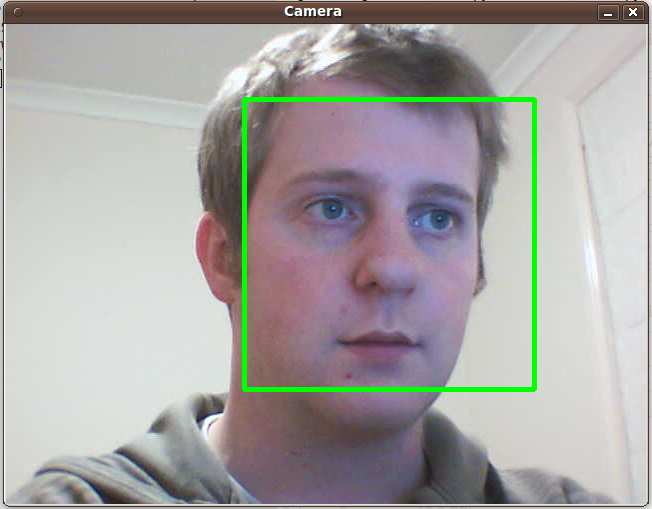
\includegraphics[width=100mm, height=80mm]{images/face-detect_square.png}
  \caption{Imagen 1}
\end{figure}

\section{Landmarks}
Para este problema hemos probado dos soluciones diferentes, ambas basadas en openCV.  

\subsection{Haar Cascades}
La primera ha sido utilizando haar cascades de los ojos y la sonrisa, lo cual no daba un resultado muy óptimo ya que a veces no era capaz de detectar ambos ojos, o no era capaz de detectar la boca. Esto causaba muchos problemas a la hora de introducir los datos en la red neuronal ya que el número de entradas no puede variar. En el caso de streaming esto era especialmente problemático ya que era más dificultoso filtrar los frames que no habían sido correctamente clasificados.

\begin{figure}[H]
  \centering
  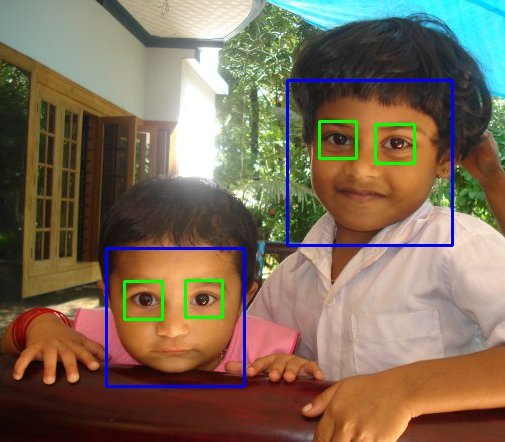
\includegraphics[width=100mm, height=80mm]{images/face_detection_haar_cascades.jpg}
  \caption{Detección de cara y ojos haar cascades}
\end{figure}

\subsection{Dlib}

\section{Algoritmo de cálculo de distancias}

\begin{figure}[H]
  \centering
  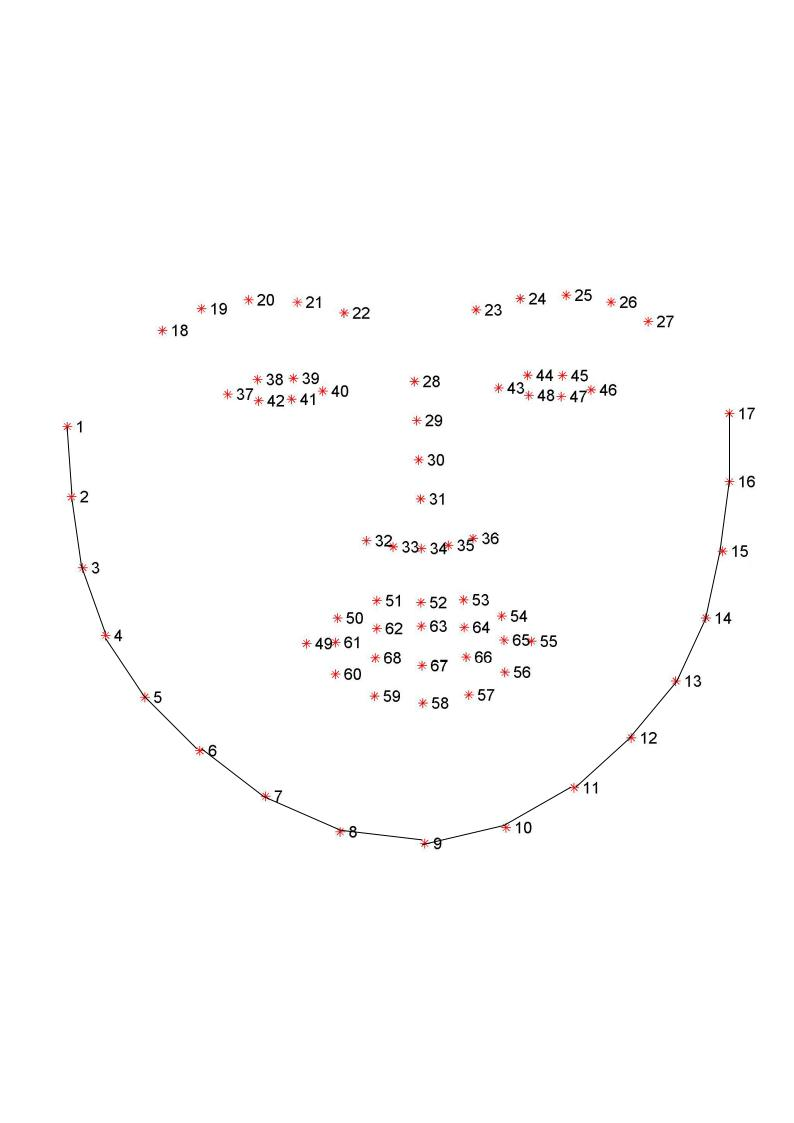
\includegraphics[width=100mm, height=80mm]{images/border_distances.jpg}
  \caption{Imagen 1}
\end{figure}


\begin{figure}[H]
  \centering
  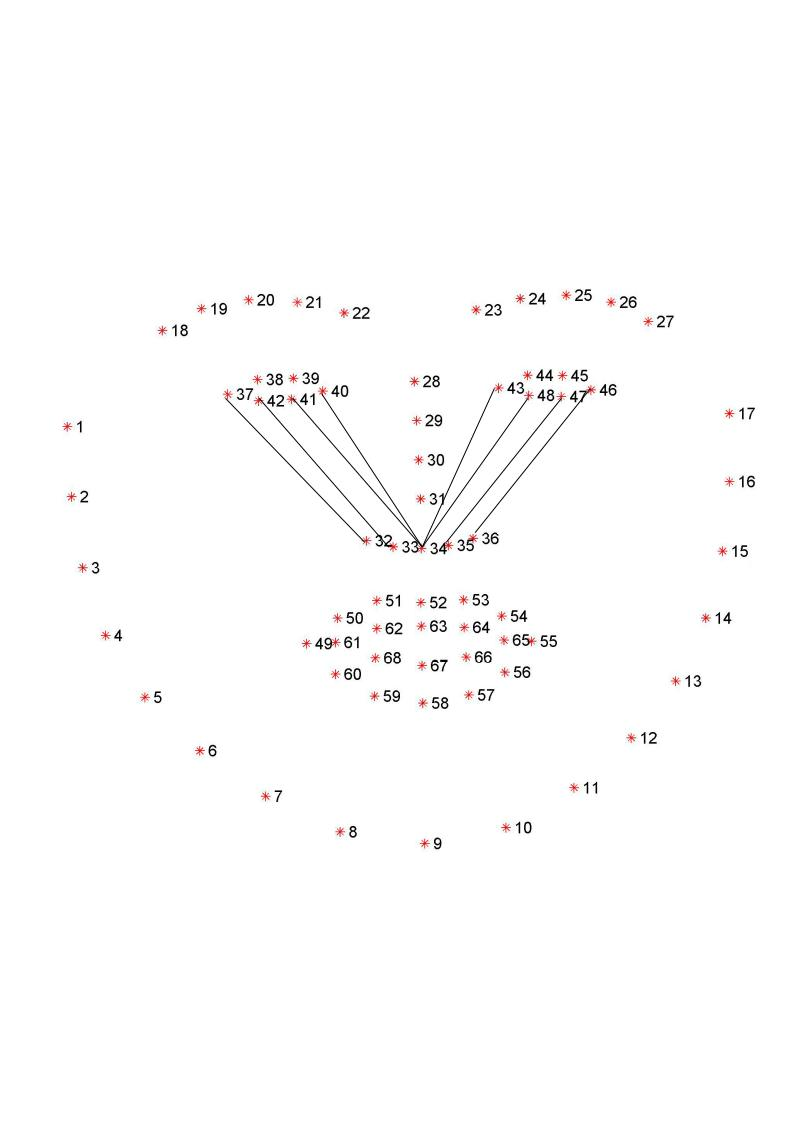
\includegraphics[width=100mm, height=80mm]{images/cheekbone_distances.jpg}
  \caption{Imagen 1}
\end{figure}


\begin{figure}[H]
  \centering
  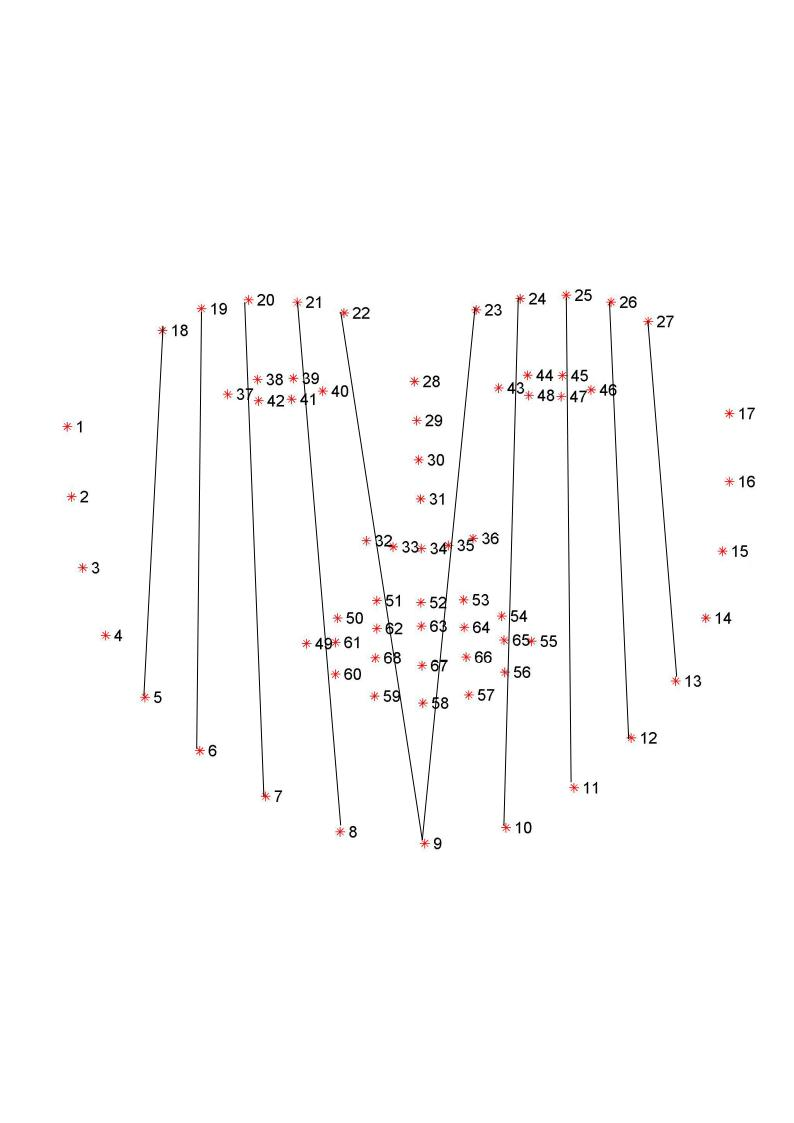
\includegraphics[width=100mm, height=80mm]{images/height_distances.jpg}
  \caption{Imagen 1}
\end{figure}


\begin{figure}[H]
  \centering
  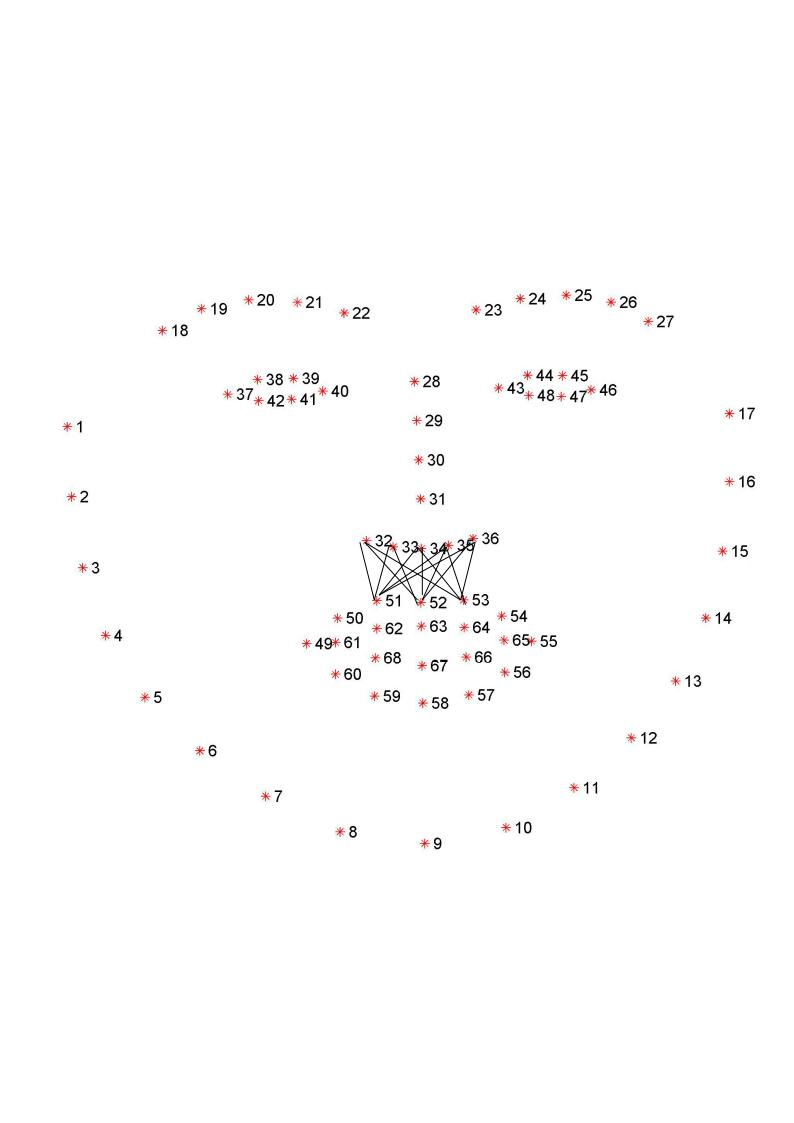
\includegraphics[width=100mm, height=80mm]{images/moustache_distances.jpg}
  \caption{Imagen 1}
\end{figure}  
  
\begin{figure}[H]
  \centering
  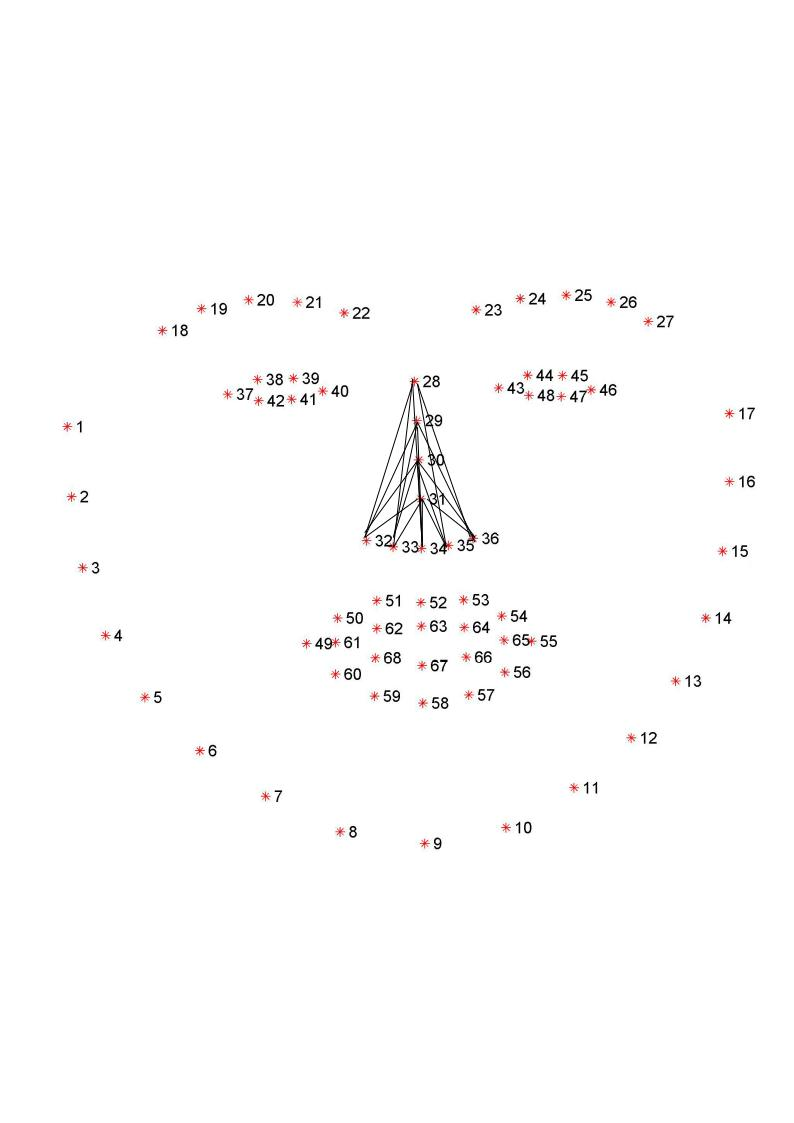
\includegraphics[width=100mm, height=80mm]{images/nasal_septum_distances.jpg}
  \caption{Imagen 1}
\end{figure}
  
\begin{figure}[H]
  \centering
  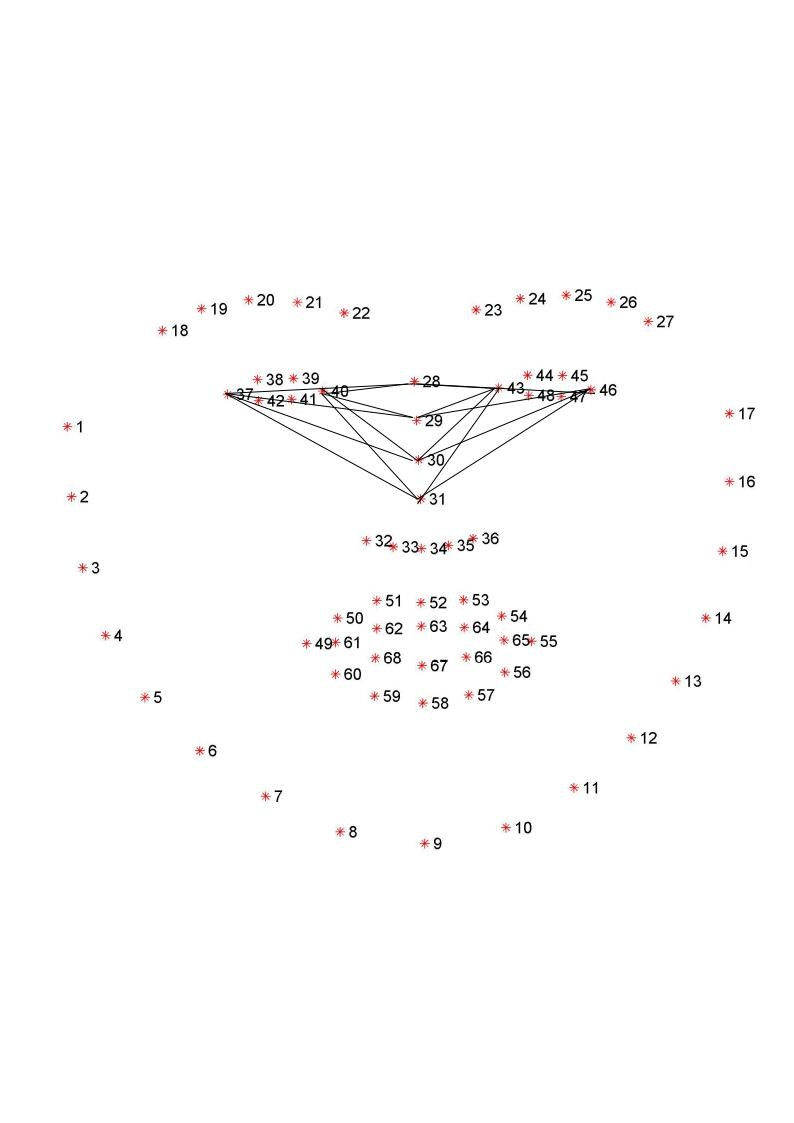
\includegraphics[width=100mm, height=80mm]{images/nose_distances.jpg}
  \caption{Imagen 1}
\end{figure} 
  
\begin{figure}[H]
  \centering
  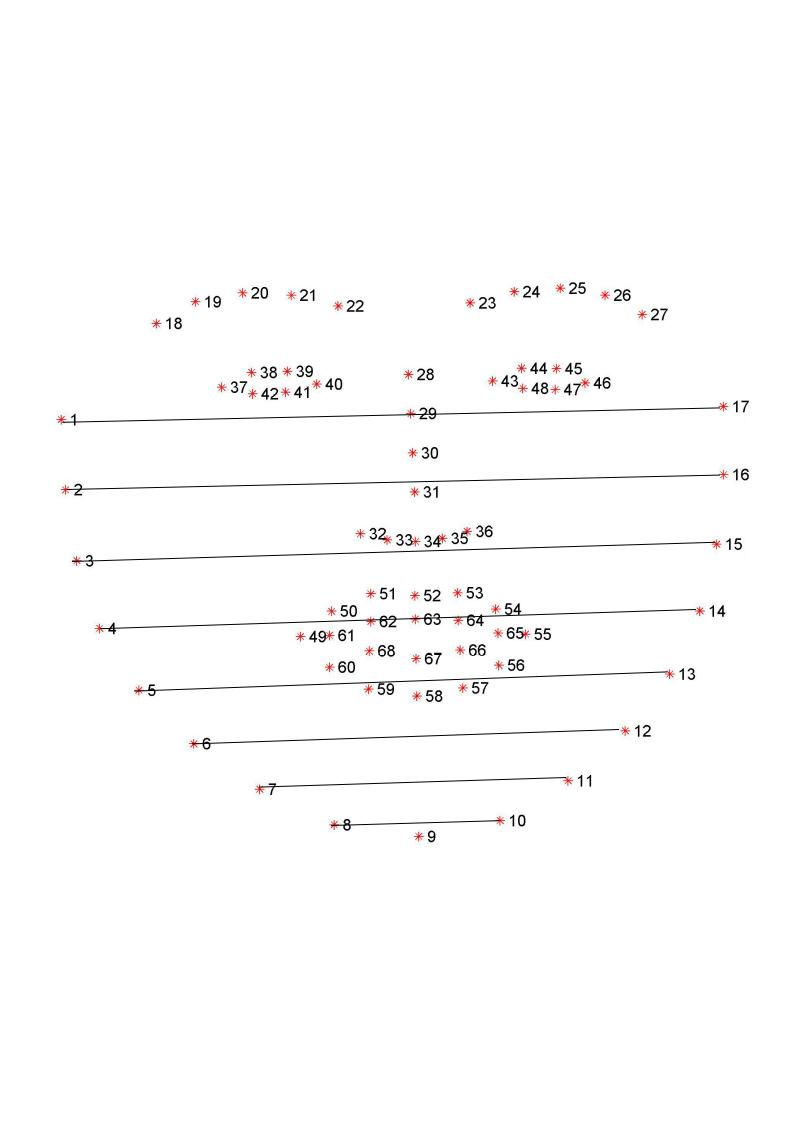
\includegraphics[width=100mm, height=80mm]{images/width_distances.jpg}
  \caption{Imagen 1}
\end{figure}

\section{Red Neuronal Multicapa}

\section{Red Neuronal Convolucional}

\section{Referencias}

\end{document}